\input{configuration}

\title{Lecture 23 --- Transaction Isolation }

\author{Jeff Zarnett \\ \small \texttt{jzarnett@uwaterloo.ca}}
\institute{Department of Electrical and Computer Engineering \\
  University of Waterloo}
\date{\today}


\begin{document}

\begin{frame}
  \titlepage

 \end{frame}



\begin{frame}
\frametitle{Transaction Isolation}
Transaction isolation: is that multiple concurrent transactions should not be able to lead somehow to an inconsistent state due to concurrent operations. 

The simple approach is to force transactions to run one at a time, which of course ensures that concurrency is not a problem... 

...but also ensures that nobody uses your database because it's very slow.

\end{frame}

\begin{frame}
\frametitle{Transaction Isolation}

\begin{center}
	
\includegraphics[width=0.6\textwidth]{images/tooslow.jpg}
\end{center}

\end{frame}



\begin{frame}
\frametitle{Threading}

The database server has the same threading problems that you likely recall from the discussion of concurrency.

The operating system schedules the threads and it chooses when it is a good time for a switch between them.

\end{frame}

\begin{frame}[fragile]
\frametitle{Back to the Bank}

One transaction is a transfer of \$50 from A to B.

Another transaction is the calculation of monthly earned interest.

{\scriptsize
\begin{multicols}{2}
\textbf{Transaction $T_{1}$}
\begin{verbatim}
T1.1. read A.balance
T1.2. A.balance = A.balance - 50
T1.3. write A.balance
T1.4. read B.balance
T1.5. B.balance = B.balance + 50
T1.6. write B.balance
\end{verbatim}
\columnbreak
\textbf{Transaction $T_{2}$}

\begin{verbatim}
T2.1 read A.balance
T2.2 A.balance = A.balance * 1.01
T2.3 write A.balance
\end{verbatim}

\end{multicols}
}

\end{frame}


\begin{frame}
\frametitle{Concurrency Problems}

 An improper interleaving of two statements means one of the changes gets lost, and the \$50 is not deducted or the interest is not calculated at all. 
 
This pair of transactions is interesting in that there are two correct answers. 
 
\$1969.50 and \$1970.00 -- a difference of 50 cents.

Both answers are correct in the sense that they are consistent.

\end{frame}

\begin{frame}
\frametitle{Scheduling}

These two execution sequences are called \alert{schedules} and they represent a chronological ordering in which instructions are executed.

A schedule is called valid if it does not break any of the rules and cannot cause some inconsistent state.

 A serial schedule means one transaction runs to completion before the next begins and for $n$ transactions there are $n!$ different valid serial schedules. 


\end{frame}

\begin{frame}
\frametitle{More Speed, More Risk}

Probably you have noticed however, that the operations on the A account are finished in $T_{1}$ after statement \texttt{T1.3}. 

You could in theory start the second transaction a little bit early to get some performance increase. 

Well -- maybe! 

\end{frame}

\begin{frame}
\frametitle{More Speed, More Risk}

That might be revealing the partial state of a transaction and that might not be acceptable. 

\begin{center}
	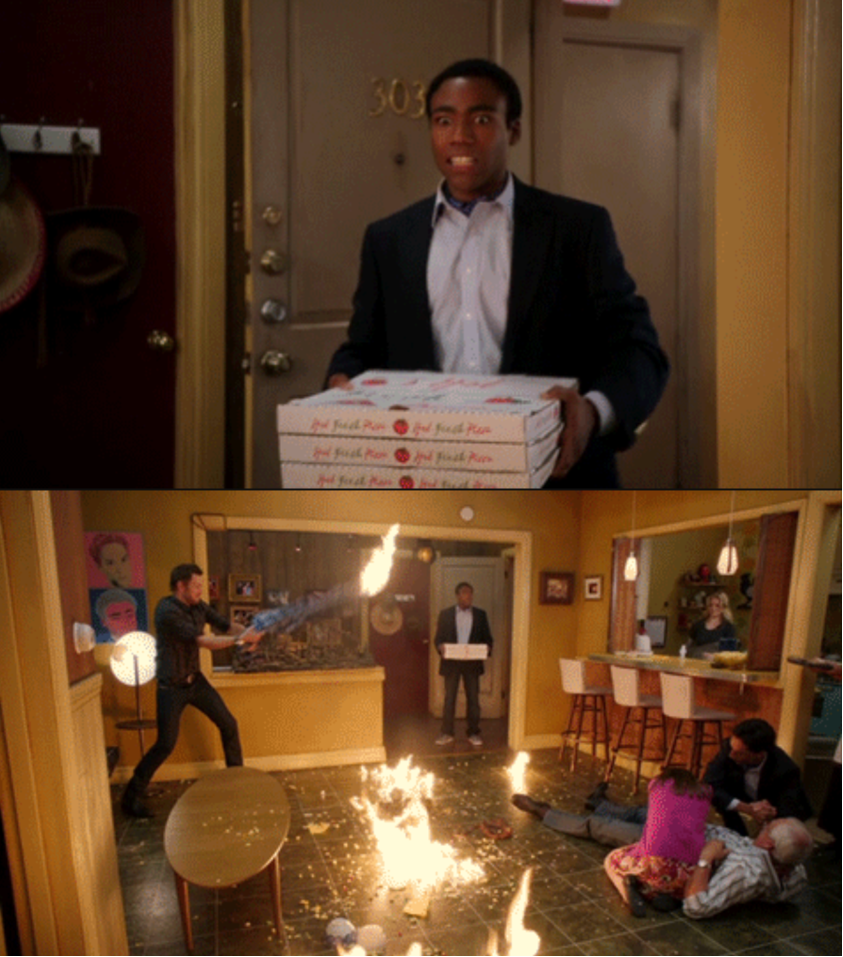
\includegraphics[width=0.4\textwidth]{images/troy.png}
\end{center}

What if an error is encountered on assigning the balance of B because and the transaction is to be rolled back? Things start to get interesting...


\end{frame}

\begin{frame}
\frametitle{Serial vs Serializable}

We do not actually need for all transactions to be done serially, but they do need to be \alert{serializable}.

This means there must exist an equivalent serial schedule.

That means the end result when all is said and done must be the same as if the transactions executed in a serial order (any serial order).

\end{frame}


\begin{frame}[fragile]
\frametitle{Serializable}

This is equivalent to the serial schedule of first $T_{1}$ and then $T_{2}$:

\begin{verbatim}
T1.1. read A.balance
T1.2. A.balance = A.balance - 50
T1.3. write A.balance
T2.1 read A.balance
T2.2 A.balance = A.balance * 1.01
T2.3 write A.balance
T1.4. read B.balance
T1.5. B.balance = B.balance + 50
T1.6. write B.balance
\end{verbatim}

\end{frame}

\begin{frame}[fragile]
\frametitle{Not Serializable}

This not okay because it does not match either $T_{1}$ then $T_{2}$ or $T_{2}$ then $T_{1}$:

\begin{verbatim}
T1.1. read A.balance
T1.2. A.balance = A.balance - 50
T2.1 read A.balance
T2.2 A.balance = A.balance * 1.01
T2.3 write A.balance
T1.3. write A.balance
T1.4. read B.balance
T1.5. B.balance = B.balance + 50
T1.6. write B.balance
\end{verbatim}

\$1950.00...

\end{frame}

\begin{frame}
\frametitle{Determining Serializability}


If our intention is to ensure serializability, we do need to know how to tell if a schedule is serializable. 

For simple examples, we can determine by inspection whether it is serializable.

When multiple transactions are interleaved it starts to get more difficult.

\end{frame}

\begin{frame}
\frametitle{Determining Serializability}


From the view of the database (or any program, really), it is more or less irrelevant what the contents of a variable or attribute are.

\begin{center}
	
\includegraphics[width=0.45\textwidth]{images/nobodycares.jpg}
\end{center}

The order reads and writes are what matter; the actual value is irrelevant.

\end{frame}

\begin{frame}
\frametitle{Beware of Hazards!}

\begin{enumerate}
	\item \textbf{RAW} (Read After Write)
	\item \textbf{WAR} (Write After Read)
	\item \textbf{WAW} (Write After Write)
	\item \textbf{RAR} (Read After Read) - No such hazard! 
\end{enumerate}

Two transactions $T_{i}$ and $T_{j}$ are said to \alert{conflict} if they are operations by different transactions on the same data... 

...and at least one of those operations is a write.

\end{frame}

\begin{frame}
\frametitle{Be Conflict-Free}

Non-conflicting instructions can swap with no consequences in the schedule. 

If a schedule $S$ can be transformed into $S'$ by a series of swaps of non-conflicting instructions, we say that $S$ and $S'$ are conflict-equivalent.

\end{frame}

\begin{frame}
\frametitle{Be Conflict-Free}

If a particular schedule $S$ is conflict-equivalent to a serial schedule then it is called conflict-serializable.

We need a particular schedule to be conflict-serializable, not serial; that is enough to make sure we can perform the operations and get consistent results.

\end{frame}

\begin{frame}
\frametitle{Determining Conflict-Serializability}

A simple approach to determining the conflict-serializability of a schedule relies on building a directed graph called a precedence graph. 

This is formed out of the transactions participating in the schedule and constraints are reflected as edges in this graph. 

\end{frame}

\begin{frame}
\frametitle{Determining Conflict-Serializability}

Each transaction is a node. 

If $T_{i}$ does a read before $T_{j}$ does a write, that is an edge from $T_{i}$ to $T_{j}$. 

The same holds for a RAW dependency and for a WAW dependency. 

\end{frame}


\begin{frame}
\frametitle{Super Simple Precedence Graphs}

\begin{center}
\includegraphics[width=0.4\textwidth]{images/precedence-1}
\includegraphics[width=0.4\textwidth]{images/precedence-2}
\end{center}

Once the precedence graph has been assembled, it is fairly easy for humans to figure out a valid serial ordering of the transactions. 

If a cycle is detected, a topological sort is not possible: it cannot be turned into a linear ordering of transactions. 

\end{frame}

\begin{frame}
\frametitle{Topological Sort}

\begin{center}
\includegraphics[width=0.35\textwidth]{images/topological}
\end{center}


\end{frame}

\begin{frame}
\frametitle{Isolation and Atomicity}

If we have a schedule that is not serial but conflict-equivalent to one, we have a potential problem that we did not have before. 

Suppose we have two transactions that are running in parallel and we have a schedule that is conflict equivalent to first $T_{1}$ then $T_{2}$. 

What if transaction $T_{1}$ writes a value, then $T_{2}$ reads that value, but $T_{1}$ aborts immediately afterwards and needs to be rolled back? 

\end{frame}

\begin{frame}
\frametitle{Recoverable}

We would like to know what schedules make recovery possible at all, and even which schedules make recovery relatively simple. 

If we can recover from a problem, the schedule is called \alert{recoverable}. 

A schedule that is not recoverable should never be chosen.

It means a transaction that is aborted could potentially result in inconsistent results, violating the atomicity principle.

\end{frame}

\begin{frame}
\frametitle{Recoverable}

On the other hand, if a transaction $T_{k}$ is committed, it should never be necessary to roll that transaction back. 

If we did, the durability property would be violated. 

What do we want?

\end{frame}

\begin{frame}
\frametitle{Recoverable}


The behaviour we are looking for in the example is that if $T_{1}$ aborts for some reason, $T_{2}$ must also abort.

\end{frame}

\begin{frame}
\frametitle{Recoverable}

The schedule is recoverable as long as no transaction $T$ commits until all transactions $T'$ that precede it have committed. 

``Precede'' in the previous sentence refers to our idea of the precedence graph.

The placement of the commit operations is what makes a schedule recoverable.

\end{frame}



\begin{frame}
\frametitle{Rollback Cascade}

If we have two transactions as above like $T_{1}$ and $T_{2}$ and the first transaction aborts, it may cause the second transaction to abort. 

But: transaction that aborts may cause some other transactions to abort, which would in turn cause more transactions to abort.

This is called a \alert{cascade rollback}.

\end{frame}

\begin{frame}
\frametitle{Cascade Rollback}

\begin{center}
	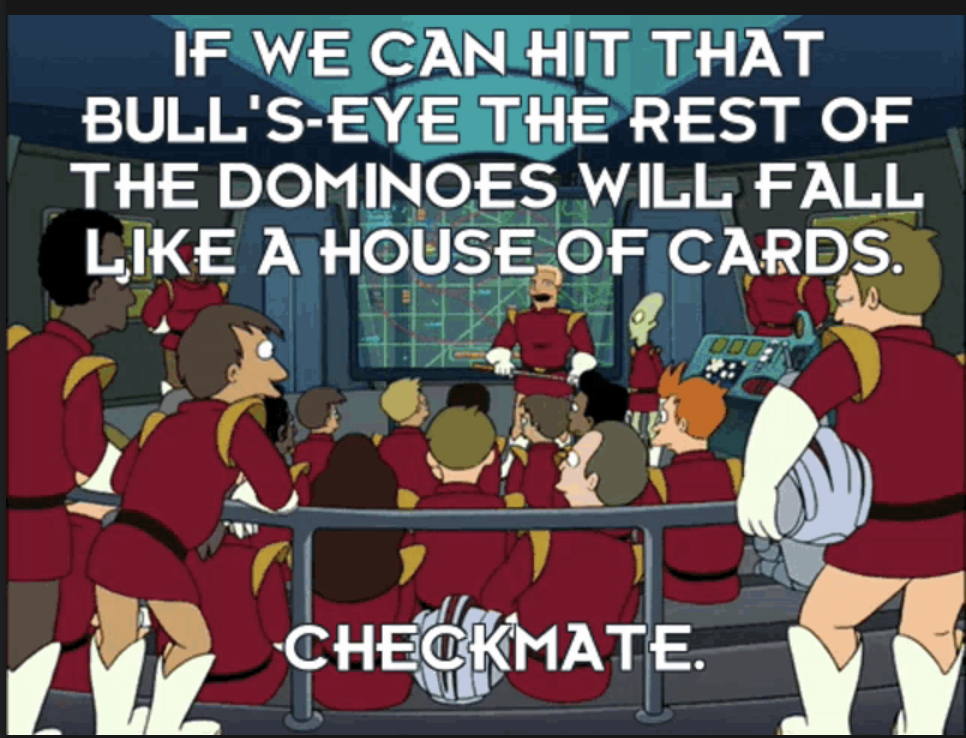
\includegraphics[width=0.75\textwidth]{images/checkmate.png}
\end{center}


\end{frame}

\begin{frame}
\frametitle{Cascadeless Schedules}

It may be desirable, where possible, to prevent the need to cascade rollbacks. 

A schedule will be \alert{cascadeless} (i.e. contain no cascade rollbacks) if every transaction only reads items that have already been committed. 

It should be easy to convince yourself that if that is the case, then a cascade rollback can never occur. 


\end{frame}

\begin{frame}
\frametitle{Strict Schedules}

There is a third, even more restrictive schedule called a \alert{strict schedule}.

In this, transactions may neither read nor write a data element until the last transaction that writes that element has committed (or aborted).

This even more restrictive schedule means that it will be relatively easy to recover if we must.

\end{frame}

\begin{frame}
\frametitle{Transaction Isolation Levels}

Serializability is how the database server ensures that data operations produce consistent results. 

As there are performance costs that come with performing things strictly, we will sometimes allow a little bit of rule-breaking to allow better performance... 

This is dangerous, and it means that more care needs to be taken on the part of the developers. 

If they want to use this sort of feature they need to be responsible about its use.


\end{frame}

\begin{frame}
\frametitle{Transaction Isolation Levels}

The isolation levels specified in the SQL standard are:
\begin{itemize}
	\item \textbf{Serializable}
	\item \textbf{Repeatable read}
	\item \textbf{Read committed}
	\item \textbf{Read uncommitted}
\end{itemize}

All isolation levels above also forbid writing a data item that has already been written by another transaction that has not yet been committed (or aborted).

\end{frame}

\begin{frame}
\frametitle{Non-Repeatable Reads}

Non-repeatable reads tend to happen in real life a lot.

Selecting seats on a flight: when you go to select seats, you are presented with a map and you get to make your choice about which seat. 

If multiple people are doing the same thing then there is no problem unless two people are trying to choose the same seat.

\end{frame}

\begin{frame}
\frametitle{Non-Repeatable Reads}


If that's not the case, then there is no conflict. 

If they are choosing the same seat, there might be a slight problem: both people cannot have the same seat.


\end{frame}

\begin{frame}
\frametitle{Non-Repeatable Reads}

Ultimately, one user will succeed and the second user will not. 

The successful user will be told of the success and the unsuccessful user will be prompted to select again, and be presented with the updated map. 

This is a form of rollback, really!


\end{frame}

\begin{frame}
\frametitle{Non-Repeatable Reads}


The user then may choose whether to give up or try again. 

In a rather unpleasant scenario, the user may be forced to try several times before succeeding.

\begin{center}
	
\includegraphics[width=0.4\textwidth]{images/seatconflict.jpg}
\end{center}

\end{frame}

\begin{frame}
\frametitle{Non-Repeatable Reads}

We could force serializability by allowing only 1 passenger to select at a time. 

That might be acceptable (if annoying) if seat selection took place only at the time when flights are booked. 


\end{frame}

\begin{frame}
\frametitle{Non-Repeatable Reads}


That isn't what happens, though; people select them at check-in. 

In that case we let the users make edits, but the process of actually updating the database runs in transactions, and those transactions need to be serialized. 

\end{frame}

\begin{frame}
\frametitle{Client-Server Database Interactions}

This problem is a general one when we have client applications interacting with data stored in the database. 

The stored data is called up and sent to the client for editing. 

If some other client is accessing that data at the same time, there is a conflict. 

\end{frame}

\begin{frame}
\frametitle{Client-Server Database Interactions}


Before changes are applied, it is common to reload the underlying data and see if it has changed. 

If so, then the current edit cannot go through without some sort of confirmation or changes.

\end{frame}

\begin{frame}
\frametitle{Achieving Isolation}

To actually achieve the isolation levels, there are three strategies: 

\begin{itemize}
\item Locking 
\item Timestamps 
\item Snapshot isolation
\end{itemize}

\end{frame}

\begin{frame}
\frametitle{Locking}

Locking is pretty much what you would expect: synchronization primitives are established and then they need to be acquired and released as is appropriate.

Suppose we have locks for each table. If we need more than one table, we have the possibility of a deadlock. 

\end{frame}

\begin{frame}
\frametitle{Locking}

Remember from the discussion of concurrency the idea of two-phase locking. 


We can also have reader-writer locks which could speed up execution of the transaction as well, especially if reads are much more common than writes.

\end{frame}

\begin{frame}
\frametitle{Timestamps}

Timestamps are pretty simple; each transaction is assigned a timestamp, typically when it begins. 

Each data item has a read-timestamp and a write-timestamp, which are updated when the item is read our written respectively. 

The database server can then ensure that transactions that conflict are executed in order of the timestamps. 

Failing that, abort (and possibly restart) the transaction.


\end{frame}

\begin{frame}
\frametitle{Snapshot Isolation}
When a transaction is to begin, a copy is made of the data needed and the copy is modified, and then finally the modified version is committed (or aborted). 

This avoids the need for locking of tables, since each transaction gets its own copy of the data.

This does have a potential drawback: too much isolation! 

If there are two concurrent transactions, it may happen that neither transaction can ``see'' the updates from the other.

\end{frame}


\end{document}

